\subsection{Pumpen}
\label{subsubsec:Pumpen}

Um die Flüssigkeit aus den Flaschen in das Glas abzufüllen, werden gemäss Kapitel \ref{subsec:Entscheidungfindung_des_Aufbaus} Pumpen eingesetzt. Es werden daher verschiedene Typen miteinander verglichen.

\subsubsection{Anforderungen}\label{par:Anforderungen_Pumpen}

\begin{tabularx}{\textwidth}{lllX}
Durchflussmenge & : & Aus Pflichtziel & min. 0.6l pro Minute\\
 & & Aus Wunschziel & min 1.2l pro Minute \\
Spannung & : & Spannungsversorgung & 12-24V \\
Schlauchanschluss & : & Innendurchmesser & 6-8mm \\
Sonstiges & : & Hygieneanforderungen & Lebensmittelpumpe \\
\end{tabularx}

\subsubsection{Mögliche Pumpen}\label{par:Mögliche_Pumpen}

Da es sich um Lebensmittel handelt welche befördert werden sollen, werden zwei verschiedene Pumpentypen verglichen. Einerseits ist dies die Schlauchpumpe, welche über ihren mechanischen Aufbau ein Vakuum erzeugt, und somit Flüssigkeit ansaugt. Der grosse Vorteil dieses Pumpentyps ist, dass diese durch den Aufbau in der Lage ist, die zu befördernde Menge zu dosieren. In Abbildung \ref{fig:Schlauchpumpe} kann der Aufbau dieses Pumpentyps betrachtet werden. \cite{acky69_schlauchpumpe_2018}

\begin{figure}[h!]
	\centering
	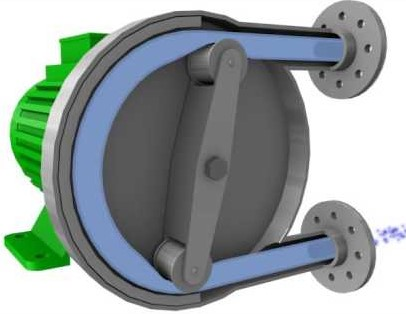
\includegraphics[width=0.6\textwidth]{graphics/Schlauchpumpe.jpg}
	\caption{Aufbau einer Schlauchpumpe \cite{creative_commons_techniker_2019}}
	\label{fig:Schlauchpumpe}
\end{figure}   

Bei jeder spezifizierten Umdrehung des Motors wird die im Schlauch befindliche Menge an Flüssigkeit zwischen zwei oder mehreren Rollen befördert. In Abbildung \ref{fig:Schlauchpumpe} ist dies nach jeder halben Umdrehung der Fall mit zwei Rollen. Werden mehrere Rollen verbaut, so kann diese Menge varriiert werden. Mit der Regelung der Drehzahl des Motors kann somit die  zu befördernde Flüssigkeitsmenge über die Zeit bestimmt werden. Eingesetzt werden diese Pumpen oft in der Medizinaltechnik, wo meist kleinere Mengen an Flüssigkeit befördert werden. Dabei kann mit einer Genauigkeit von weniger als 1\% gerechnet werden. Werden grössere Flussraten benötigt, so steigt die Ungenauigkeit dieses Pumpentyps. So muss bei einer Flussrate von 800 ml/min mit einer Abweichung von $\pm$ 8\% gerechnet werden. Um diese Ungenauigkeit beheben zu können, müsste ein externes Durchflussmessgerät installiert werden. \cite{acky69_schlauchpumpe_2018}  

Beim zweiten Pumpentyp handelt es sich um einen weiteren Typ einer Vakuumpumpe, genauer gesagt eine Membranpumpe. Bei diesem Pumpentyp wird mittels Rotation über Gummimembranen ein Vakuum erzeugt, welches das zu befördernde Medium über ein Einwegventil einsaugt und über ein weiteres Einwegventil wieder abgibt. Eine solche Pumpe ist in Abbildung \ref{fig:Membranpumpe} zu sehen. \cite{jens_uber_die_felder_membranpumpe_2019}

\begin{figure}[h!]
	\centering
	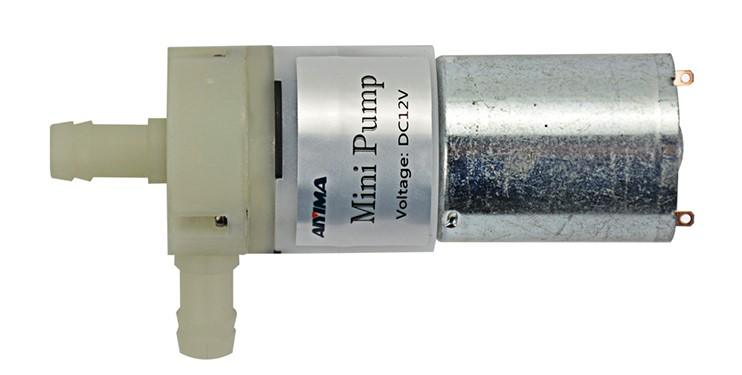
\includegraphics[width=0.6\textwidth]{graphics/Membranpumpe.jpg}
	\caption{Ansichtbild einer Membranpumpepumpe \cite{aiyimaindustrial_store_us_nodate}}
	\label{fig:Membranpumpe}
\end{figure}  

Der grosse Vorteil dieses Pumpentyps ist die hohe Lebensdauer sowie der geringe Preis. Auch bei diesem Pumpentyp kann mittels Drehzahl über die Zeit die zu befördernde Menge berechnet werden. Dies weist jedoch auch nicht die erforderliche Genauigkeit gemäss dem Pflichtenheft auf. Desshalb muss auch bei diesem Pumpentyp eine externe Durchflussmessung durchgeführt werden. \cite{jens_uber_die_felder_membranpumpe_2019}\\

\begin{table}[h!]
\begin{tabularx}{\textwidth}{|X|X|}
\hline
\textbf{Schlauchpumpe:} & \textbf{Membranpumpe:}
\\
\hline
- Spannung: 24V & - Spannung: 12V \\

- Sromverbrauch: ca. 700mA & - Sromverbrauch: <600mA\\

- Durchfluss: bis 800ml/min & - Durchfluss: 1000-1500ml/min\\

- Messung des Durchflusses: extern & - Messung des Durchflusses: extern\\

- Preis der verglichenen Pumpe: 70.86\$  & - Preis der verglichenen Pumpe: 6.37\$\\

- Bestellseite: Aliexpress & - Bestellseite: Aliexpress\\

\hline
\end{tabularx}
\caption{Vergleich der zwei Pumpentypen \cite{aiyimaindustrial_store_us_nodate}\cite{dongguan_honlite_industrial_co._ltd._800_nodate}}
\end{table}

\subsubsection{Verwendete Pumpe}\label{par:Verwendete_Pumpe}

Beide Pumpen entsprechen mindestens den Wunschzielen gemäss dem Pflichtenheft. Allerdings ist die mechanische Abnutzung beider Pumpentypen verschieden. So wird bei der Schlauchpumpe der Schlauch relativ stark beansprucht, was zur Folge hat, dass dieser mit der Zeit ausgewechselt werden muss. Die Membranpumpe hingegen bietet da eine höhere Lebensdauer. Der grösste Unterschied bietet jedoch der Preis. Da die Schlauchpumpe mehr als 10 Mal so viel kostet, wie die Membranpumpe und davon 12stk. benötigt werden, wird die Membranpumpe eingesetzt. Ausserdem kann mit der Schlauchpumpe nur das Pflichtziel gemäss Pflichtenheft umgesetzt werden und mit der Membranpumpe auch das Wunschziel. 